\section{理论方法}

\subsection{分栏显示}
\begin{frame}{经典的双栏显示,一边图片一边文字}
    \begin{columns}
        \begin{column}{0.5\textwidth}
            人为分栏可通过columns语法实现\\
            双栏的宽度比例可以通过参数调整\\

        \end{column}
        \begin{column}{0.5\textwidth}
            \begin{figure}[h]
                \centering
                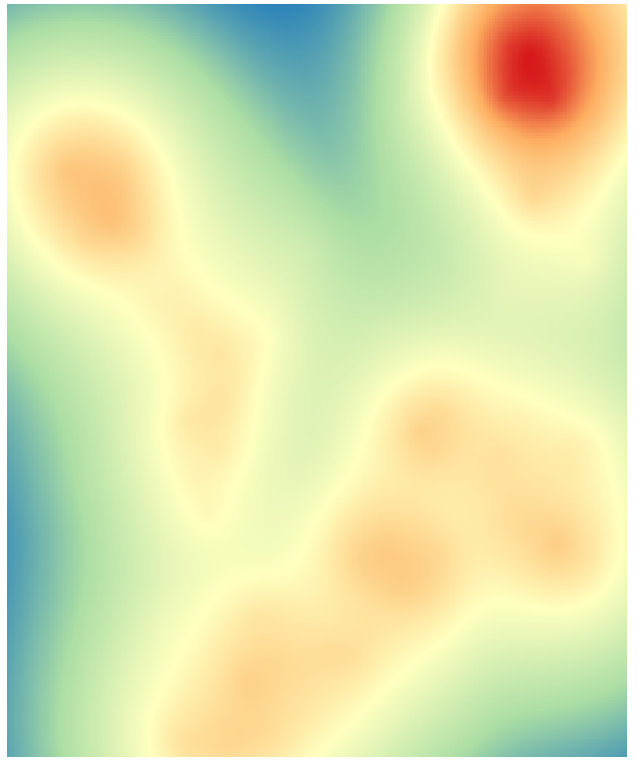
\includegraphics[width=0.5\textwidth]{images/example.png}
                \caption{一张简单的图片示例}
                \label{fig:3dtiles}
            \end{figure}
        \end{column}
    \end{columns}
\end{frame}

\subsection{列表}
\begin{frame}{不带编号的列表}
    使用itemize环境,使用item命令添加列表项
    \begin{itemize}
        \item 1
        \item 2
        \item 3
    \end{itemize}
\end{frame}

\begin{frame}{带有编号的列表}
    使用enumerate环境,使用item命令添加列表项
    \begin{enumerate}
        \item 1
        \item 2
        \item 3
    \end{enumerate}
\end{frame}

\subsection{数学公式}
\begin{frame}{数学公式}
    简单的数学公式使用\$...\$包裹,复杂的公式使用equation环境
    \begin{equation}
        \label{eq:1}
        \sum_{i=1}^n a_i=0
    \end{equation}
\end{frame}